\documentclass[a4paper,12pt]{article}
\usepackage[utf8]{inputenc}
\usepackage{graphicx}
\usepackage{graphics}
\usepackage{hyperref}
\usepackage{geometry}
\usepackage{float}
% \usepackage{comment}
\graphicspath{ {build/} } 
\geometry{left=2cm, right=2cm, top=2cm, bottom=2cm}

\begin{document}

\begin{titlepage}
    \begin{center}
        \vspace*{3cm}
        
        {\Huge \textbf{Laboratorio 2 - Grupo 7}}\\[1cm]
        {\LARGE Panel solar automático:\\ [0.5cm]  Selección de Hardware, Diagrama de bloques, periféricos, comunicaciones.}\\[2cm]
        
        \vfill
        
        {\Large \textbf{Integrantes }}\\[.5cm]
        \large
        \begin{tabular}{c c}
            Gartner, Francisco Nehuen & 69864/6 \\
            Marchesotti, Guido Daniel & 69923/9 \\
            Rosa, Fausto Pablo & 69843/1 \\
        \end{tabular}
        
        \vspace{1cm}
        
        \begin{figure}[b]
            \centering
            
\includegraphics[width=1\linewidth]{LOGOSFI-UNLP-color-01.png}
        \end{figure}
        
        %%{\large \today}
    \end{center}
\end{titlepage}

%%\newpage
%%\tableofcontents
%%\newpage

A continuación se especificaran los posibles componentes a utilizar, así como las especificaciones y criterios tenidos en cuenta para elegirlos. \\
Los componentes necesarios serán: 
\begin{itemize}
\item Microcontrolador
\item Sensor de Potencia
\item Sensor de Luz
\item Motores
\item Panel Solar
\item Regulador de Carga
\item Batería
\item Transmisor inalámbrico
\end{itemize}

En \hyperref[fig:diagrama]{figura 1} se puede observar un diagrama de bloques con su conexionado. 

\begin{figure}[H]
    \centering
    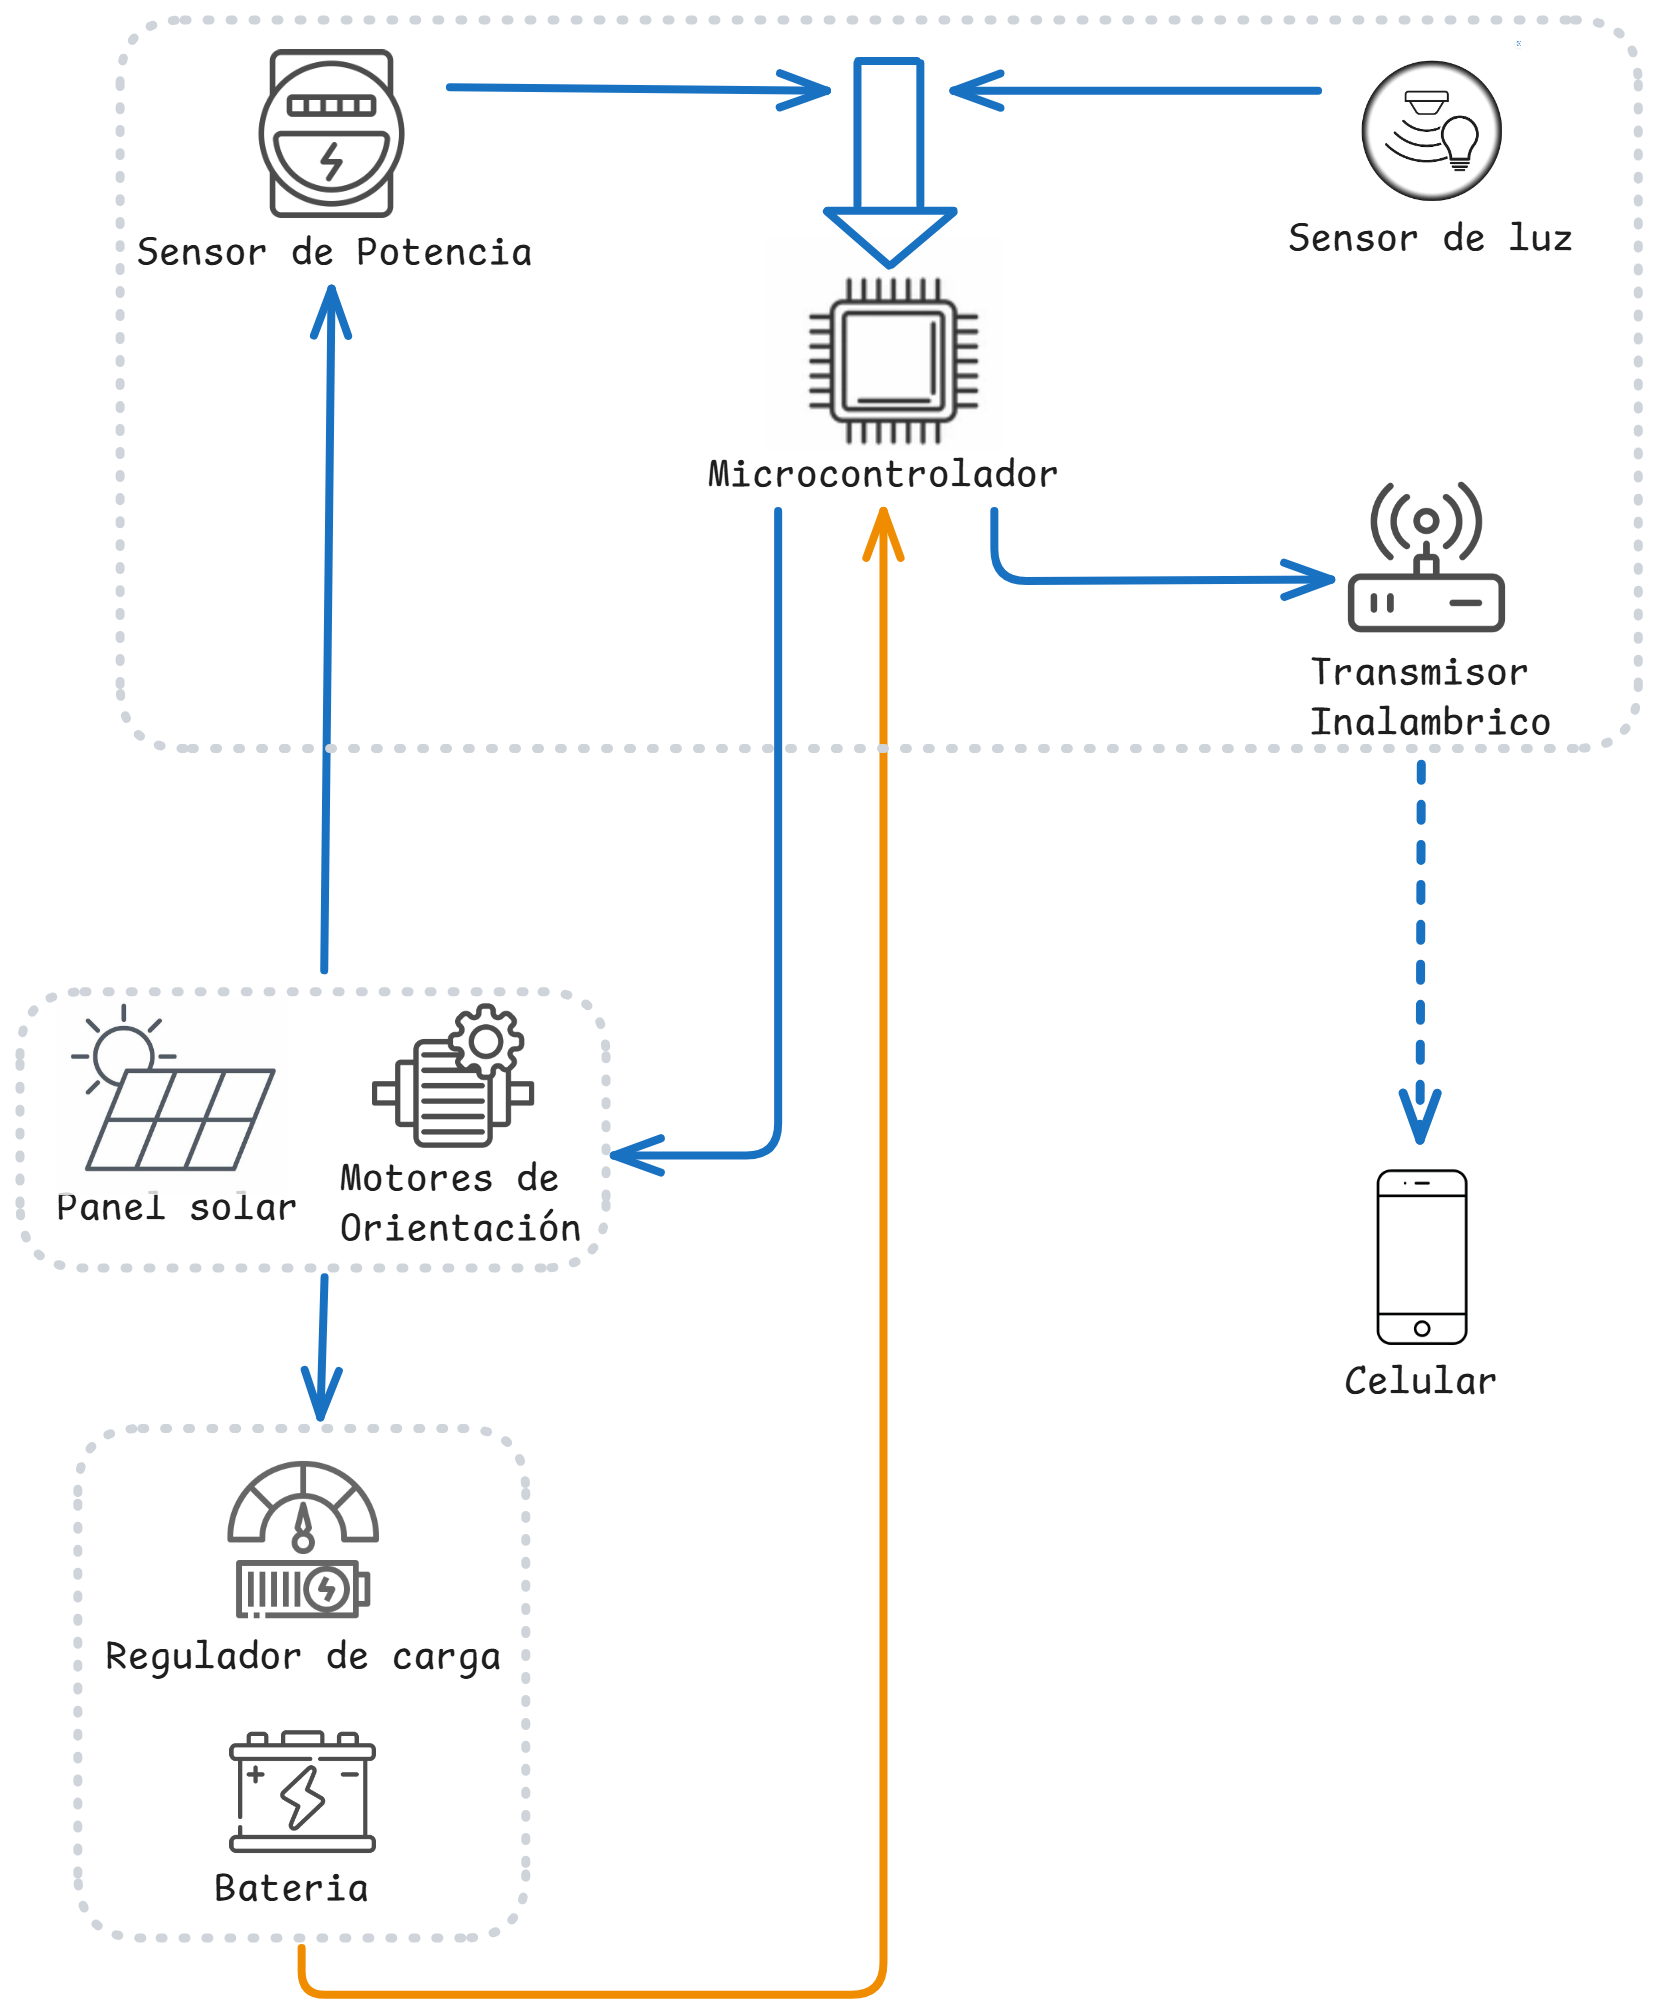
\includegraphics[width=0.75\linewidth]{diagrama_proyecto.png}
    \caption{ diagrama de bloques de los componentes generales}
    \label{fig:diagrama}
\end{figure}


Cabe aclarar que en la selección de todos los componentes se tuvo en cuenta la disponibilidad y el precio siendo estas importantes limitaciones en el desarrollo del trabajo practico

Microcontrolador: 
Dentro del proyecto tenemos limitaciones impuestas para la elección del microcontrolador. Aún así, se pueden nombrar algunas características destacables del mismo que se ajustan a las tareas a realizar. Como el sistema de seguimiento solar no requiere una acción de control rápida, la transmisión de datos no requiere de una velocidad elevada y los calculos a realizar son de bajo consto computacional, se puede elegir un microcontrolador de características moderadas. Esto nos permitirá disminuir el consumo de energía alcanzando un mayor eficiencia energética, característica importante en sistemas  dependientes de baterías. Además, el Atmega328p es un microcontrolador popular con amplias librerías ya desarrolladas y funcionales.\\

Sensor de Potencia: 
Considerando las características del panel solar, contando con una potencia máxima de 10 Watts, una corriente de de cortocircuito de 0.57A y un voltaje de circuito abierto de 23.5V se opta por componentes con un rango capaz de abarcar estos limites impuestos por el panel. Se tomaron en cuenta criterios como la sencillez de uso, al ser capaz de sensar múltiples variables con un único componente, la precisión y el consumo. A su vez, se pensó en la disponibilidad en el país y el costo. 
Debido a la lenta variación de la potencia, no se ha priorizado en la velocidad de muestreo a la hora de barajar entre los posibles componentes.\\ 

INA 219\\
Modulo Sensor Tension Corriente Max471 Para Arduino Emakers\\
Sensor Corriente Shunt 3ch Ina3221 Smbus I2c Itytarg\\
ac712\\

Sensor de Luz:
Para el sensor de luz, que se utilizará para seleccionar la dirección del panel, se eligieron cuatro foto-resistores. Se eligió esta configuración donde se comparan los valores de los cuatro foto-resistores por ser usada en proyectos similares. \\

Motores:
Para la elección de los motores que moverán al panel en dirección acimutal y vertical (altura solar), se tomó en cuenta la potencia de los motores así como el torque necesario para ambas tareas. El primero será el de más uso, ya que el panel deberá rotar entre 120° y -120° por lo menos una vez al día, mientras que el segundo debe ser capaz de levantar el peso total del panel en dirección vertical. AGREGAR ESPECIFICACION PASO A PASO (PRECISIÓN) \\

Panel solar:
El panel solar es pieza clave del proyecto y el que determinará la potencia máxima generable. Para su selección se tomó en cuenta la potencia máxima, su corriente de salida nominal, su tensión de salida nominal y qué reguladores de carga eran compatibles con el mismo, siendo esta una de las condiciones más limitantes. RESISTENCIA INTEMPERIE (CONDICIÓN NO FUNCIONAL), HUMO\\

Panel Solar 10w 12v Luxen Policristalino Energia Solar\\

Regulador de carga:
Como se mencionó con anterioridad, el regulador de carga debió se elegido en conjunto con el panel solar teniendo en cuenta condiciones como la tensión de salida nominal del mismo. Pero fuera de las especificaciones técnicas, la característica de mayor relevancia es el costo. La tecnología del regulador de carga elegido es PWM, siendo esta una tecnología simple y barata que permite extraer energía del panel de manera efectiva a un relativo bajo costo. Esto comparado con otros sistemas que usan MPPT (maximum power point tracking) de mayor eficiencia en la extracción pero con un costo muy superior, inviable para proyectos a pequeña escala. PROTECCIONES DEL PANEL Y BATERÍA. TENSIÓN DE SALIDA (ALIMENTACIÓN DEL MICRO), SOLUCIONA CARGA TE BATERIA, [EXTRACCION DEL PANEL Y ALIMENTACIÓN DEL SISTEMA]\\

Batería:
mAH QUE PUEDE ENTREGAR, VOLTAJE CONDICIONADO POR EL REGULADOR DE CARGA, 

Transmisor inalámbrico:
La transmisión de datos en esta actividad no requiere se rápida, pero si eficiente. Al depender el sistema de la energía almacenada en las baterías, es necesario que el emisor pueda conectarse a la interfaz gráfica de manera inalámbrica sin comprometer la integridad de los datos, de manera eficiente y sin agotar la batería. Además, se planea que la distancia máxima a la que se deben trasmitir los datos almacenados no debe superar los 10 metros. ESPECIFICAR LOS TIPOS DE COMUNICACIÓN, I2C, \\
HC-05 GW-040 \\

\begin{table}[H]
\centering
    \begin{tabular}{|l|c|c|r|}
    \hline
    \textbf{Característica} & \textbf{Opción A} & \textbf{Opción B} & \textbf{Opción C} \\
    \hline
    Elemento 1 & Valor A1 & Valor B1 & Valor C1 \\
    \hline
    Elemento 2 & Valor A2 & Valor B2 & Valor C2 \\
    \hline
    Elemento 3 & Valor A3 & Valor B3 & Valor C3 \\
    \hline
    Elemento 4 & Valor A4 & Valor B4 & Valor C4 \\
    \hline
    \end{tabular}
    \caption{Comparativa entre Opción A, B y C}
    \label{tab:comparativa}
\end{table}

\end{document}
